\documentclass[UTF8,zihao=-4,fontset=none,a4paper]{ctexart}
\setCJKmainfont[BoldFont={Droid Sans Fallback}]{Droid Sans Fallback}
\setCJKsansfont[BoldFont={Droid Sans Fallback}]{Droid Sans Fallback}
\setCJKmonofont{Droid Sans Fallback}

\usepackage[left=24mm,right=24mm,top=22mm,bottom=23mm]{geometry}
\usepackage{amsmath,amssymb,bm}
\usepackage{graphicx}
\usepackage{booktabs,tabularx,array}
\usepackage{xcolor}
\usepackage{caption}
\usepackage{fancyhdr}
\usepackage[unicode,colorlinks=true]{hyperref}

\definecolor{nornblue}{HTML}{173B65}
\definecolor{norngray}{HTML}{536171}
\definecolor{nornlight}{HTML}{EEF3F8}
\hypersetup{linkcolor=nornblue,urlcolor=nornblue,citecolor=nornblue,
  pdftitle={NORN：年代不确定性感知与物理一致性约束的全球古地壳厚度重建},
  pdfsubject={中文 Methods：模型框架、年代观测算子、物理约束与联合反演}}
\ctexset{section={format=\Large\bfseries\color{nornblue}},
  subsection={format=\large\bfseries\color{nornblue}}}
\captionsetup{font=small,labelfont=bf}
\pagestyle{fancy}
\fancyhf{}
\fancyhead[L]{\small\color{norngray}NORN\quad 中文 Methods}
\fancyhead[R]{\small\color{norngray}框架、公式与联合反演}
\fancyfoot[C]{\small\thepage}
\setlength{\headheight}{16pt}
\setlength{\parskip}{0.3em}
\setlength{\emergencystretch}{2em}
\renewcommand{\arraystretch}{1.25}
\linespread{1.12}
\allowdisplaybreaks[2]
\newcommand{\dif}{\mathop{}\!\mathrm{d}}
\newcommand{\divs}{\nabla_s\!\cdot}
\newcommand{\loss}{\mathcal{L}}

\title{\vspace{-1.2em}\color{nornblue}\bfseries NORN：年代不确定性感知与物理一致性约束的全球古地壳厚度重建}
\author{\large Methods 中文说明}
\date{}

\begin{document}
\maketitle
\vspace{-2.4em}

NORN 将全球古地壳厚度重建表述为一个受观测和物理约束的时空反演问题：利用年代条件的球面神经网络表示厚度历史，通过古厚度记录、现代厚度数据以及运动学和体积收支关系共同约束模型。物理公式依次通过预测厚度场、计算物理残差、构造联合损失和更新参数参与反演。

\noindent\colorbox{nornlight}{\parbox{\dimexpr\linewidth-2\fboxsep\relax}{\small
\textbf{适用范围与实现状态。}本文介绍图~\ref{fig:framework} 所示的完整方法设计。当前训练流程已实现 SFNO、年代混合似然和现代厚度约束；古轨迹采样及物理损失仍待接入。本文中的物理模块说明不代表已经完成相应训练或验证。
}}

\begin{figure}[htbp]
  \centering
  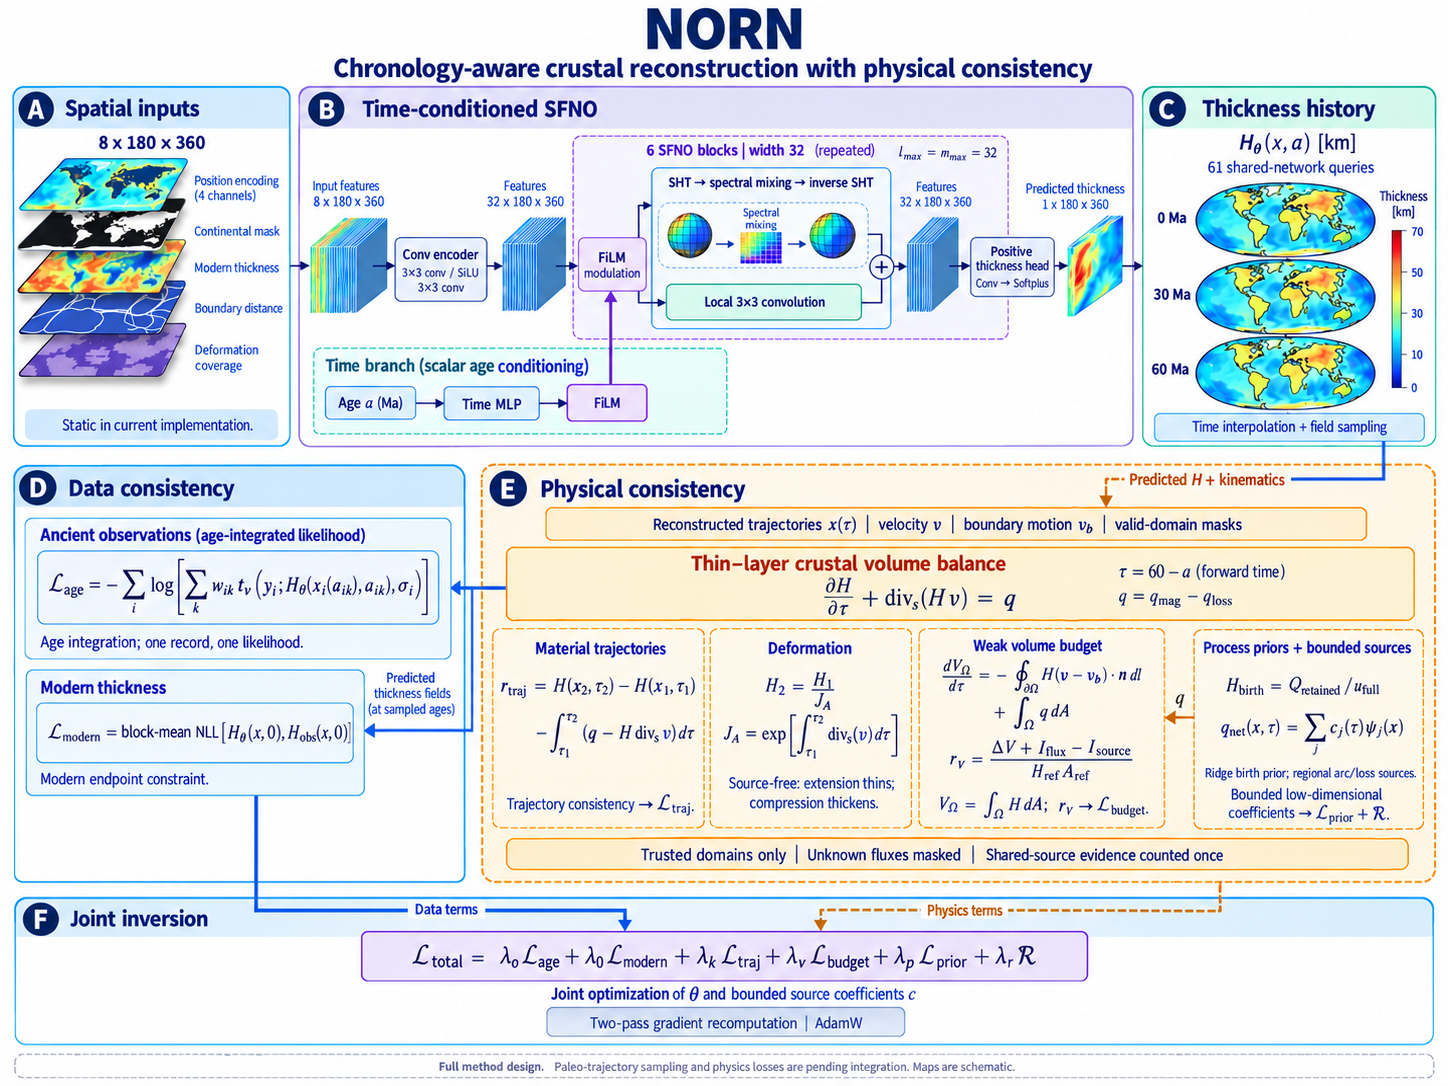
\includegraphics[width=\linewidth]{figures/norn_framework.png}
  \caption{NORN 完整方法框架。A--C：空间输入、年代条件 SFNO 与厚度历史；D：古观测和现代端点的数据约束；E：薄层地壳运动学、轨迹一致性、变形关系、弱形式体积预算及过程先验；F：联合优化。虚线物理分支表示待接入的设计。图中地图颜色仅作示意。}
  \label{fig:framework}
\end{figure}

\clearpage
\section{研究目标与问题定义}

设 $x\in\mathbb{S}^2$ 为球面位置，$a\in[0,60]$ 为地质年龄，单位为 Ma。模型估计地壳正厚度场 $H_\theta(x,a)$，单位为 km，其中 $\theta$ 表示网络参数。现代厚度数据约束当前状态，古厚度记录约束历史状态，板块运动与体积收支关系则限制观测稀疏区域内允许出现的演化方式。

NORN 是针对给定观测集合的实例型反演求解器。网络提供厚度场的可微参数化，历史观测通过优化目标约束其参数。模型没有将任意观测集合编码为单次前向重建的观测编码器，因此更换观测集合通常需要重新优化。

为统一记号，表~\ref{tab:symbols} 汇总主要变量。物理方程采用向现代推进的时间 $\tau=60-a$，其单位为 Myr。下文的 $H(x,\tau)$ 表示同一厚度场在该时间坐标下的表达，即 $H(x,\tau)=H_\theta(x,60-\tau)$。

\begin{table}[htbp]
  \centering
  \caption{主要符号及含义。}
  \label{tab:symbols}
  \small
  \begin{tabularx}{\linewidth}{@{}lXl@{}}
    \toprule
    符号 & 含义 & 单位或说明 \\
    \midrule
    $x,\ a,\ \tau$ & 球面位置、地质年龄、向前物理时间 & $\tau=60-a$ \\
    $H_\theta$ & 网络表示的正地壳厚度 & km \\
    $\mathbf v,\ \mathbf v_b$ & 材料切向速度、控制域边界速度 & km/Myr \\
    $q$ & 净厚度源项，$q_{\rm mag}-q_{\rm loss}$ & km/Myr \\
    $J_A$ & 两个时刻之间的水平面积伸展比 & 无量纲 \\
    $V_\Omega$ & 控制域 $\Omega$ 内的地壳体积 & km$^3$ \\
    $y_i,\ \sigma_i$ & 第 $i$ 条古厚度记录及误差尺度 & km \\
    $a_{ik},\ w_{ik}$ & 年龄积分节点及其权重 & $\sum_k w_{ik}=1$ \\
    $c_j,\ \psi_j$ & 区域源项的低维系数与空间基函数 & 乘积具有源项单位 \\
    \bottomrule
  \end{tabularx}
\end{table}

\section{年代条件的球面厚度场表示}

\subsection{空间输入与 SFNO 主干}

当前神经主干使用 $8\times180\times360$ 的空间特征张量，包括位置编码、大陆掩膜、现代厚度、板界距离和变形区覆盖信息。当前实现对所有年代使用同一份空间输入；完整设计中的运动学资料还拟用于古位置查询和物理约束计算。

卷积编码器首先将输入映射到 32 个隐藏通道，随后通过 6 个 SFNO 模块。每个模块包含球谐谱分支和局部卷积分支。谱分支依次进行球谐变换、谱系数通道混合和逆变换，采用 $l_{\max}=m_{\max}=32$ 的截断设置，并结合残差与归一化操作；局部 $3\times3$ 卷积分支用于补充局部空间结构。

年代 $a$ 经小型多层感知机编码为时间特征，并通过 FiLM 产生通道缩放和偏移参数。该机制使同一组网络权重能够表示不同地质年代的厚度场。输出头使用正值变换：
\begin{equation}
  H_\theta(x,a_m)
  =\operatorname{softplus}\!\left(F_\theta(X,a_m)(x)\right)+\epsilon,
  \label{eq:field}
\end{equation}
其中，$X$ 为输入特征，当前实现取 $\epsilon=0.5\ \mathrm{km}$。模型只输出一通道厚度，不采用自由逐像素噪声输出头。

\subsection{时间锚点与连续年龄查询}

模型在 $a_m=0,1,\ldots,60\ \mathrm{Ma}$ 上生成 61 张锚点厚度图。在允许插值的区间内，非整数年龄通过相邻锚点查询：
\begin{equation}
  H_\theta(x,a)=\sum_m b_m(a)H_\theta(x,a_m),
  \qquad b_m(a)\geq0,\quad\sum_m b_m(a)=1.
  \label{eq:interpolation}
\end{equation}
相邻锚点的 $b_m$ 为线性插值权重。所有时刻共享网络参数并联合拟合，上一时刻预测图不作为下一时刻的必需输入。对完整物理设计，拓扑事件附近需要分段、单侧处理或有效性屏蔽，不能默认跨事件插值始终可靠。

\section{年代不确定性感知的观测建模}

\subsection{古厚度记录的年龄边缘似然}

古厚度记录通常具有年龄区间 $[a_i^{\min},a_i^{\max}]$。NORN 将真实年龄视为潜在变量，在允许的年龄分布内对观测似然进行积分。对第 $i$ 条厚度记录 $y_i$，采用加权求积近似：
\begin{equation}
  p(y_i\mid\theta)
  \approx\sum_{k=1}^{K_i}w_{ik}\,
  t_\nu\!\left(y_i;\mu_{ik},\sigma_i\right),
  \qquad\sum_{k=1}^{K_i}w_{ik}=1,
  \label{eq:mixture}
\end{equation}
\begin{equation}
  \mu_{ik}=H_\theta\!\left(x_i(a_{ik}),a_{ik}\right),
  \qquad
  \loss_{\rm age}=-\frac{1}{N_{\rm tr}}
  \sum_{i\in\mathcal I_{\rm tr}}\log p(y_i\mid\theta).
  \label{eq:age-loss}
\end{equation}
这里，$t_\nu(y;\mu,\sigma)$ 表示以 $\mu$ 为位置参数、$\sigma$ 为尺度参数的 Student-t 分布；$\mathcal I_{\rm tr}$ 为训练记录集合，$N_{\rm tr}$ 为其数量。均值归一化仅决定损失尺度，可与联合目标中的权重相配合。

当前实现取 $\nu=4$：点年龄使用 1 个节点，宽度不超过 5 Myr 的非零年龄区间使用 3 个节点，更宽区间使用 8 个节点。Student-t 似然用于降低异常记录的影响。误差尺度按记录或来源设定，不允许自由逐点增大噪声以消除拟合误差。

式~\eqref{eq:mixture} 保证每条观测仅贡献一个似然项。增加年龄节点只改善积分精度，不会把同一记录转化为多条独立证据。完整设计中的 $x_i(a)$ 表示由经过核验的板块重建模型得到的古位置；当前训练脚本仍按现代坐标取样，这一实现差异必须在使用结果时明确。

\subsection{现代端点约束}

现代厚度通过高斯负对数似然约束 $H_\theta(x,0)$。为减少密集空间采样对损失的支配，当前实现先计算空间块内平均，再对空间块取平均：
\begin{equation}
  \loss_{\rm modern}
  =\frac{1}{B}\sum_{b=1}^{B}\frac{1}{|\mathcal B_b|}
  \sum_{j\in\mathcal B_b}
  \left[
    \frac{\big(H_\theta(x_j,0)-H_j^{\rm obs}\big)^2}{2\sigma_{0j}^{,2}}
    +\frac{1}{2}\log\!\left(2\pi\sigma_{0j}^{,2}\right)
  \right].
  \label{eq:modern}
\end{equation}
其中，$\mathcal B_b$ 为第 $b$ 个空间块，$\sigma_{0j}$ 为现代观测的指定误差尺度。现代数据作为带误差的观测参与优化，而不是处处强制成立的精确真值。

\section{薄层地壳运动学与物理一致性}

本节对应图~\ref{fig:framework} 的物理分支，描述拟接入的完整约束。在相同参考密度的薄层近似下，采用地壳体积形式的输运关系，避免将不同密度地壳的体积收支直接等同于严格质量守恒。

\subsection{厚度输运与源汇平衡}

采用向现代推进的时间 $\tau$，控制方程为
\begin{equation}
  \frac{\partial H}{\partial\tau}
  +\divs(H\mathbf v)
  =q,\qquad q=q_{\rm mag}-q_{\rm loss}.
  \label{eq:balance}
\end{equation}
其中，$\mathbf v$ 为球面切向速度，$q_{\rm mag}$ 和 $q_{\rm loss}$ 分别表示增加和损失厚度的过程。式~\eqref{eq:balance} 将厚度变化与材料输运、水平面积变形和净源汇联系起来。若改用地质年龄 $a$，对应形式为 $-\partial H/\partial a+\divs(H\mathbf v)=q$，时间导数前的负号不能省略。

该关系适用于具有运动学支持的薄层近似域。显著下地壳侧向流、多层叠置等过程若无法由采用的表面运动学表达，需要引入受限模型差异或降低约束强度。

\subsection{材料轨迹一致性}

沿经过核验的存活材料轨迹，厚度变化满足
\begin{equation}
  \begin{aligned}
  r_{\rm traj}={}&H(x_2,\tau_2)-H(x_1,\tau_1)\\
  &-\int_{\tau_1}^{\tau_2}
  \left(q-H\divs\mathbf v\right)\dif\tau .
  \end{aligned}
  \label{eq:trajectory}
\end{equation}
轨迹残差用于构造 $\loss_{\rm traj}$，约束模型预测的厚度变化与沿途源汇和变形相容。在无源、无面积变形的可靠刚性板块内，式~\eqref{eq:trajectory} 退化为沿轨迹厚度近似不变。该结论不扩展到所有构造域，也不要求板块边界两侧厚度连续。

\subsection{面积变形与增减厚关系}

在无源、近似不可压缩条件下，面积伸展比 $J_A$ 与厚度满足
\begin{equation}
  H_2=\frac{H_1}{J_A},
  \qquad
  J_A=\exp\!\left(
  \int_{\tau_1}^{\tau_2}\divs\mathbf v\dif\tau
  \right).
  \label{eq:deformation}
\end{equation}
因此，$J_A>1$ 对应面积伸展和厚度减薄，$J_A<1$ 对应面积压缩和厚度增加。这里的 $J_A$ 是两个时刻之间的面积比，不能在每个时间步重复使用相同累计伸展因子。

式~\eqref{eq:deformation} 是同一输运机制在特定条件下的表达。若其先验与轨迹或体积预算来自同一份运动学资料，应共享证据预算或选择适当约束形式，避免将相同信息重复视为独立证据。

\subsection{弱形式体积预算}

对于边界以速度 $\mathbf v_b$ 移动的控制域 $\Omega(\tau)$，定义地壳体积
\begin{equation}
  V_\Omega(\tau)=\int_{\Omega(\tau)}H\dif A.
\end{equation}
对应的体积收支为
\begin{equation}
  \frac{\dif V_\Omega}{\dif\tau}
  =-\oint_{\partial\Omega}
  H(\mathbf v-\mathbf v_b)\cdot\mathbf n\dif l
  +\int_\Omega q\dif A,
  \label{eq:weak-budget}
\end{equation}
其中，$\mathbf n$ 为控制域边界的外法向。对时间区间积分后，构造无量纲预算残差
\begin{equation}
  r_V=
  \frac{\Delta V+I_{\rm flux}-I_{\rm source}}
       {H_{\rm ref}A_{\rm ref}},
  \label{eq:budget-residual}
\end{equation}
\begin{align}
  I_{\rm flux}
  &=\int_{\tau_1}^{\tau_2}
  \oint_{\partial\Omega(\tau)}
  H(\mathbf v-\mathbf v_b)\cdot\mathbf n\dif l\dif\tau,\\
  I_{\rm source}
  &=\int_{\tau_1}^{\tau_2}
  \int_{\Omega(\tau)}q\dif A\dif\tau.
\end{align}
分子中的各项均具有 km$^3$ 的单位；$H_{\rm ref}A_{\rm ref}$ 为固定的参考体积尺度。区域预算用于构造 $\loss_{\rm budget}$，优先在可信的板内、变形域或可追踪材料块上计算。

俯冲消亡和洋中脊出生应通过相应边界通量或条件处理，不能假定全球活动地壳体积恒定。重要通量未知时，应屏蔽该完整预算，或改用带误差的局部约束。拓扑事件附近采用分段积分，区域身份中断时不直接跨期相减。相较在板界不连续处计算全局强形式微分，弱形式强调可核验的区域体积收支。

\section{过程先验与受限源项}

过程先验用于约束厚度演化中的未知输入与源汇。对于满足适用条件的正常洋壳出生区，出生厚度可写为
\begin{equation}
  H_{\rm birth}=\frac{Q_{\rm retained}}{u_{\rm full}},
  \label{eq:ridge}
\end{equation}
其中，$Q_{\rm retained}$ 为每单位脊长的保留熔体体积产率，单位为 km$^2$/Myr；$u_{\rm full}$ 为总扩张速度，单位为 km/Myr。缺少充分熔融资料时，该关系提供带误差的出生先验，而不是精确厚度标签。

区域净源项拟采用低维表示：
\begin{equation}
  q_{\rm net}(x,\tau)=\sum_j c_j(\tau)\psi_j(x),
  \label{eq:source}
\end{equation}
其中，$\psi_j$ 限定源汇的空间作用范围，$c_j$ 为少量区段或时间基函数系数。其幅值、符号和时间变化受到独立资料与正则项约束，避免自由逐像素源项抵消任意厚度误差。

厚度资料通常难以分别识别总生产、保留比例和损失，主设计优先约束有明确含义的净源或保留产率组合。相同来源的源项先验、派生厚度先验与预算关系应统一记账；例如，使用某个产率的参数先验及其条件预算后，不再将同一产率推导的厚度增量作为额外独立观测。

\section{数据与物理的联合反演目标}

完整方法将观测、运动学和物理预算写入同一个目标：
\begin{equation}
  \begin{aligned}
  \loss_{\rm total}={}&
  \lambda_o\loss_{\rm age}
  +\lambda_0\loss_{\rm modern}\\
  &+\lambda_k\loss_{\rm traj}
  +\lambda_v\loss_{\rm budget}
  +\lambda_p\loss_{\rm prior}
  +\lambda_r\mathcal R.
  \end{aligned}
  \label{eq:joint}
\end{equation}
数据项要求预测与古记录及现代厚度相容，轨迹和预算项限制允许的演化方式，过程先验及 $\mathcal R$ 限制源项幅值、时间变化和模型差异。权重应在训练或验证侧确定，不能根据最终测试结果反复调整。

物理融合的具体计算路径是：先由 SFNO 生成厚度场，再用外部运动学和低维源项计算轨迹与体积预算残差，将其转化为损失，与数据项共同更新 $\theta$ 及受限系数 $c$。增加物理配点或加密网格主要用于改善积分精度，不应自动增加同源先验的证据量。不同控制域和相关约束之间需要固定的归一化与证据预算。

\textbf{当前实现边界：}现有训练脚本实际使用
\begin{equation}
  \loss_{\rm current}=\loss_{\rm age}+0.5\loss_{\rm modern}.
  \label{eq:current}
\end{equation}
式~\eqref{eq:joint} 中其余项是完整设计的一部分，尚不能作为当前训练已经满足物理一致性的证据。

\section{优化实现与结果解释}

针对 61 个时间锚点，当前实现采用两遍梯度重计算。第一遍固定网络参数生成锚点场，并将缓存场 $U_m$ 视为独立可微变量，计算完整损失及
\begin{equation}
  G_m=\frac{\partial\loss}{\partial U_m}.
\end{equation}
第二遍在相同参数下重新生成锚点场，通过链式法则累积网络梯度：
\begin{equation}
  \nabla_\theta\loss
  =\sum_m
  \left(\frac{\partial H_\theta^{(m)}}{\partial\theta}\right)^{\!\top}G_m.
  \label{eq:gradient}
\end{equation}
两遍之间不更新参数，所有场相关梯度汇总后再执行优化器更新。若目标还包含直接依赖网络参数的正则项，其梯度需要另行计入；受限源项系数也按联合目标计算相应梯度。训练使用 AdamW；日志记录原始目标值，而非用于重计算反传的代理内积。

模型输出可按 $1^\circ$ 空间网格和 1 Myr 时间间隔采样，但这种输出间距不等于独立验证的地质分辨率。实际可辨识的时空尺度仍受古观测覆盖、年龄误差、代理观测语义、运动学误差及物理约束适用范围影响。当前模型输出的是单一正厚度场；年代混合似然处理观测年龄不确定性，本身并不提供已校准的历史厚度置信区间。

对于缺少观测或不具备可靠物理支持的区域，应区分数据约束、先验主导和欠约束结果。该框架的目标是给出与已有证据相容的历史重建，而不是保证全部过去具有唯一解。

\end{document}
